\paragraph{Question 1}
La complexité est de $O(m(n+m))=O(n^4)$ car~:
\begin{itemize}
\item La taille de la coupe augmente d'un sommet à chaque tour, donc
il nous faut $m$ étapes pour trouver la coupe maximum.
\item À chaque tour, on rajoute un également toutes les arêtes
incidentes au sommet rajouté.
\end{itemize}

\paragraph{Question 2}

\paragraph{Question 3}

Nous pouvons construire l'instance ci-dessous pour laquelle la borne de
deux est atteinte. 

\begin{figure}[h!]
\centering
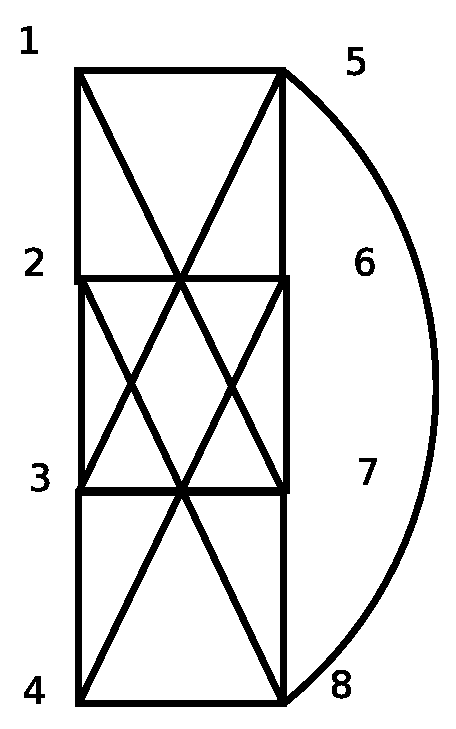
\includegraphics[height = 4cm]{../images/exo4.eps}
\caption{Instance où la borne de $2$ est atteinte, exercice 4}
\end{figure}
